\section*{2.2 More Methods of Proof}
\addcontentsline{toc}{section}{2.2 More Methods of Proof}

\subsection*{Proof by Contradiction (Indirect Proof)}
\addcontentsline{toc}{subsection}{Proof by Contradiction (Indirect Proof)}

A \textbf{proof by contradiction}, or an indirect proof, establishes $p \rightarrow q$ by assuming the hypothesis $p$ is true and that the conclusion $q$ is false and then, using $p$ and $\lnot q$ as well as other axioms, definitions, previously derived theorems, and rules of inference to derive a \textbf{contradiction}.  Basically, we derive $r \land \lnot r$ and then conclude that $q$ is true.\\

Note that
\begin{align*}
    p \rightarrow q \equiv (p \land \lnot q) \rightarrow (r \land \lnot r)
\end{align*}

\subsubsection*{Example 1}

Give a proof by contradiction of the following statement:
\begin{center}
    For every $n \in \textbf{Z}$, if $n^2$ is even, then $n$ is even.
\end{center}

Since it is not clear how to get from $n^2 = 2k_1$ to $n = 2k_2$ with a direct proof, we will try a proof by contradiction and assume $n$ is \textit{odd}.

\begin{table}[h]
\centering
\begin{tabular}{l}
$n^2$ is even (Hypothesis)\\
$n = 2k + 1$ ($k$ is an integer)\\
$n^2 = (2k + 1)^2 = 4k^2 + 4k + 1 = 2(2k^2 + 2k) + 1$\\
$n^2$ is odd. (Contradiction)\\
$n$ is odd (Conclusion)
\end{tabular}
\end{table}

From the proof, we have deduced that $n^2$ is odd, which \textit{contradicts} our hypothesis that $n^2$ is even.  Thus, we have derived $r \land \lnot r$, where 
\begin{center}
    $r: \text{$n^2$ is even}$.
\end{center}

\subsubsection*{Example 2}

Give a proof by contradiction of the following statement:
\begin{center}
    For all real numbers $x$ and $y$, if $x + y \geq 2$, then either $x \geq 1$ or $y \geq 1$.
\end{center}

We will assume the conclusion, $x \geq 1 \vee y \geq 1$ is false, so by De Morgan's law of logic, our conclusion will be

\[
    \lnot(x \geq 1 \vee y \geq 1) \equiv \lnot(x \geq 1) \land \lnot(y \geq 1) \equiv (x < 1) \land (y < 1)
\]

We add the two inequalities and obtain
\begin{center}
    x + y < 1 + 1 = 2
\end{center}

We have derived a contradition: $x + y < 2$ and $x + y \geq 2$.


\subsubsection*{Example 3}

Prove by contradiction that $\sqrt{2}$ is irrational.

$\sqrt{2}$ is irrational (Hypothesis)
\begin{align*}
\sqrt{2} &= \frac{p}{q} \text{ ($p$ and $q$ are integers and are not both even)}\\
2 &= \frac{p^2}{q^2}\\
2q^2 &= p^2 \text{ ($p^2$ is even, therefore $p$ is even, so $p = 2k$)}\\
2q^2 &= (2k)^2 = 4k^2\\
q^2 &= 2k^2 \text{ ($q^2$ is even, therefore $q$ is even)}
\end{align*}
$\sqrt{2}$ is rational (Conclusion)

From our proof, we derive that both $p$ and $q$ are even, which contradicts our assumption that $p$ and $q$ are not both even.

\subsection*{Proof by Contrapositive}
\addcontentsline{toc}{subsection}{Proof by Contrapositive}

Recall that the contrapositive of the conditional proposition $p \rightarrow q$ is $\lnot q \rightarrow \lnot p$ and both are logically equivalent.  In a \textbf{proof by contrapositive}, we prove that $\lnot q \rightarrow \lnot p$.

\subsubsection*{Example 4}

Use a proof by contrapositive to show that
\begin{center}
    For all $x \in \textbf{R}$, if $x^2$ is irrational, then $x$ is irrational.
\end{center}

Since we are using a proof by contrapositive, we want to prove that
\begin{center}
    If $x$ is rational, then $x^2$ is rational.
\end{center}

If $x$ is rational, then $x = \frac{p}{q}$ for some integers $p$ and $q$.

\begin{table}[h]
\centering
\begin{tabular}{l}
$x$ is rational (Hypothesis)\\
$x = \frac{p}{q}$ ($x$ is rational, $p$ and $q$ are integers)\\
$x^2 = \frac{p^2}{q^2}$\\
$x^2$ is rational (Conclusion)
\end{tabular}
\end{table}

\subsection*{Proof by Cases}
\addcontentsline{toc}{subsection}{Proof by Cases}

\textbf{Proof by cases} is used when the original hypothesis naturally divides itself into various cases.  If $p$ is equivalent to $p_1 \vee p_2 \vee \dots \vee p_n$ (where $p_1, p_2, \dots, p_n$ are the cases), instead of proving $(p_1 \vee p_2 \vee \dots \vee p_n) \rightarrow q$, we prove

\[
    (p_1 \rightarrow q) \land (p_2 \rightarrow q) \land \dots \land (p_n \rightarrow q).
\]

Sometimes the number of cases to prove is finite, so we check them all at once with an \textbf{exhaustive proof}.

\subsubsection*{Example 5}

Using proof by cases, prove that $2m^2 + 3n^2 = 40$ has no solutions in positive integers.\\

If $2m^2 + 3n^2 = 40$, then $m$ and $n$ are restricted in size.  In other words,
\begin{align*}
    2m^2 &\leq 40,\\
    3n^2 &\leq 40.
\end{align*}

Therefore,
\begin{align*}
    m^2 &\leq 20,\\
    n^2 &\leq \frac{40}{3} \approx 13.33.
\end{align*}

From this, we can see that $m$ can be at most 4 (because when $m = 5$, $m^2 = 25$, which is not less than 20).  Additionally, $n$ can be at most 3.  Thus, it suffices to check the cases
\begin{align*}
    m &= 1, 2, 3, 4\\
    n &= 1, 2, 3.
\end{align*}

\begin{figure}[h]
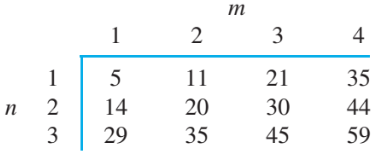
\includegraphics[width=8cm]{./02/02/proof-by-cases-table}
\centering
\end{figure}

Since $2m^2 + 3n^2 \neq 40$ for $m = 1, 2, 3, 4$ and $n = 1, 2, 3$, and $2m^2 + 3n^2 > 40$ for $m > 4$ or $n > 3$, $2m^2 + 3n^2 = 40$ has no solutions in positive integers.

\subsection*{Proofs of Equivalence}
\addcontentsline{toc}{subsection}{Proofs of Equivalence}

Theorems in the form ``$p$ if and only if $q$'', or $p \leftrightarrow q$ are proved using the logical equivalence

\[
    (p \rightarrow q) \land (q \rightarrow p).
\]

In other words, two propositions must be proved.

\subsubsection*{Example 6}

Prove that for every integer $n$, $n$ is odd if and only if $n - 1$ is even.\\

Let
\begin{align*}
    p &: n \text{ is odd},\\
    q &: n - 1 \text{ is even}.
\end{align*}

\clearpage

We first prove $p \rightarrow q$:

\begin{table}[h]
\centering
\begin{tabular}{l}
$n$ is odd (Hypothesis)\\
$n = 2k + 1$ ($k$ is an integer)\\
$n - 1 = (2k + 1) - 1 = 2k$\\
$n - 1$ is even (Conclusion)
\end{tabular}
\end{table}

Now, we prove $q \rightarrow p$:

\begin{table}[h]
\centering
\begin{tabular}{l}
$n - 1$ is even (Hypothesis)\\
$n - 1 = 2k$ ($k$ is an integer)\\
$n = 2k + 1$\\
$n$ is odd (Conclusion)
\end{tabular}
\end{table}

Some theorems state that three or more statements are logically equivalent.  To prove that $p_1, p_2, \dots, p_n$ are equivalent, we must prove

\[
    (p_1 \rightarrow p_2) \land (p_2 \rightarrow p_3) \land \dots \land (p_{n-1} \rightarrow p_n) \land (p_n \rightarrow p_1).
\]

\subsection*{Existence Proofs}
\addcontentsline{toc}{subsection}{Existence Proofs}

A proof of $\exists x P(x)$ is called an \textbf{existence proof}.  To prove it, we must find one $x$ such that $P(x)$ is true.

\subsubsection*{Example 7}

Let $a$ and $b$ be real numbers with $a < b$.  Prove that there exists a real number $x$ satisfying $a < x < b$.\\

It suffices to find one real number $x$ satisfying $a < x < b$.  The real number is

\[
    x = \frac{a + b}{2}.
\]

\subsubsection*{Example 8}

Prove that there exists a prime $p$ such that $2^p - 1$ is not prime.\\

By trial and error, we find that $2^p - 1$ is prime for $p = 2, 3, 5, 7$ but not $p = 11$.  Thus, $p = 11$ makes the statement true.

\subsubsection*{Example 9}

Let

\[
    A = \frac{s_1 + s_2 + \dots + s_n}{n}
\]

be the average of the real numbers $s_1 + s_2 + \dots + s_n$.  Prove that there exists $i$ such that $s_i \geq A$.  By proof of contradiction, we assume the negation of the conclusion, which is $\forall i (s_i < A)$.

\begin{table}[h]
\centering
\begin{tabular}{l}
there exists $i$ (Hypothesis)\\
$s_1 + s_2 + \dots + s_n < nA$\\
$\frac{s_1 + s_2 + \dots + s_n}{n} < A$\\
$\forall i (s_i < A)$ (Conclusion)
\end{tabular}
\end{table}